\section{Conclusion}
\label{sec:conclusion}

This laboratory provided us the opportunity to understand how the envelope detector and voltage regulator circuits work and also, how to improve their efficieny. We're also able to analyse carefully the working principle of an AC/DC converter. \par
In order to analyse the circuit theoreticaly \textit{Ocatve} was used as well as all the Kirchoff's equations and diode models that support this analysis. 
The simulation was done using \textit{Ngspice}. \par
Finally, we are going to compare the results from simulation and theoretical analysis side by side: \par
%compararações

\begin{center}
  \begin{tabular}{ | c | c | }
    \hline    
    {\bf Name} & {\bf Value} \\ \hline
    \section{Conclusion}
\label{sec:conclusion}

This assignment made us understand how a band pass filter work and how an OP-AMP circuit relates to and the band and the voltage gain.\par
As it can be noticed, there are some differences between the theoretical and simulation values obtained, this is the case for the OP analysis and also the impedances. This difference is explained by the use of non-linear components (transistors) that make the OP analysis deviate from the theoretical analysis. Since the linear components have constant circuit parameters, it is really easy for Ngspice to plot and analyse them in perfection in relationship to the theorethical calculations. It cannot be said the same thing for non-linear components, once those circuit parameters vary. \par
The merit figure as explained before was a very important part of this assignment, since it provides a relation with the "real world" where everything as a cost and a energy consumption, so it was important that this value was the most accurate as possible. In order to achieve that, the Ngspice's result was used. \par
As it can be way easier to compare, it is shown below the results from simulation and theoretical analysis side by side: \par
%compararações

\section{Visual Data}
\label{sec:data}

\begin{center}
  \begin{tabular}{ | c | c | }
    \hline    
    {\bf Name} & {\bf Value} \\ \hline
    merit & 1.580376e-03\\ \hline

  \end{tabular}
  \captionof{figure}{Merit Figure Table}
\end{center}

\begin{center}
  \begin{tabular}{ | c | c | }
    \hline    
    {\bf Name} & {\bf Value [$Hz$ or $dB$]} \\ \hline
    central & 9.973752e+02\\ \hline
voltagegain & 3.650113e+01\\ \hline

    \hline
  \end{tabular}
  \captionof{figure}{Central Frequency, Voltage Gain - Simulation}
\end{center}

\begin{center}
  \begin{tabular}{ | c | c | }
    \hline    
    {\bf Name} & {\bf Value [$Hz$ or $dB$]} \\ \hline
    Central Frequency & 8.141678e+02 \\ \hline 
Voltage Gain dB & 3.964755e+01 \\ 

    \hline
  \end{tabular}
  \captionof{figure}{Central Frequency, Voltage Gain - Theoretical}
\end{center}

\begin{figure}[H]
    \minipage{0.45\textwidth}
      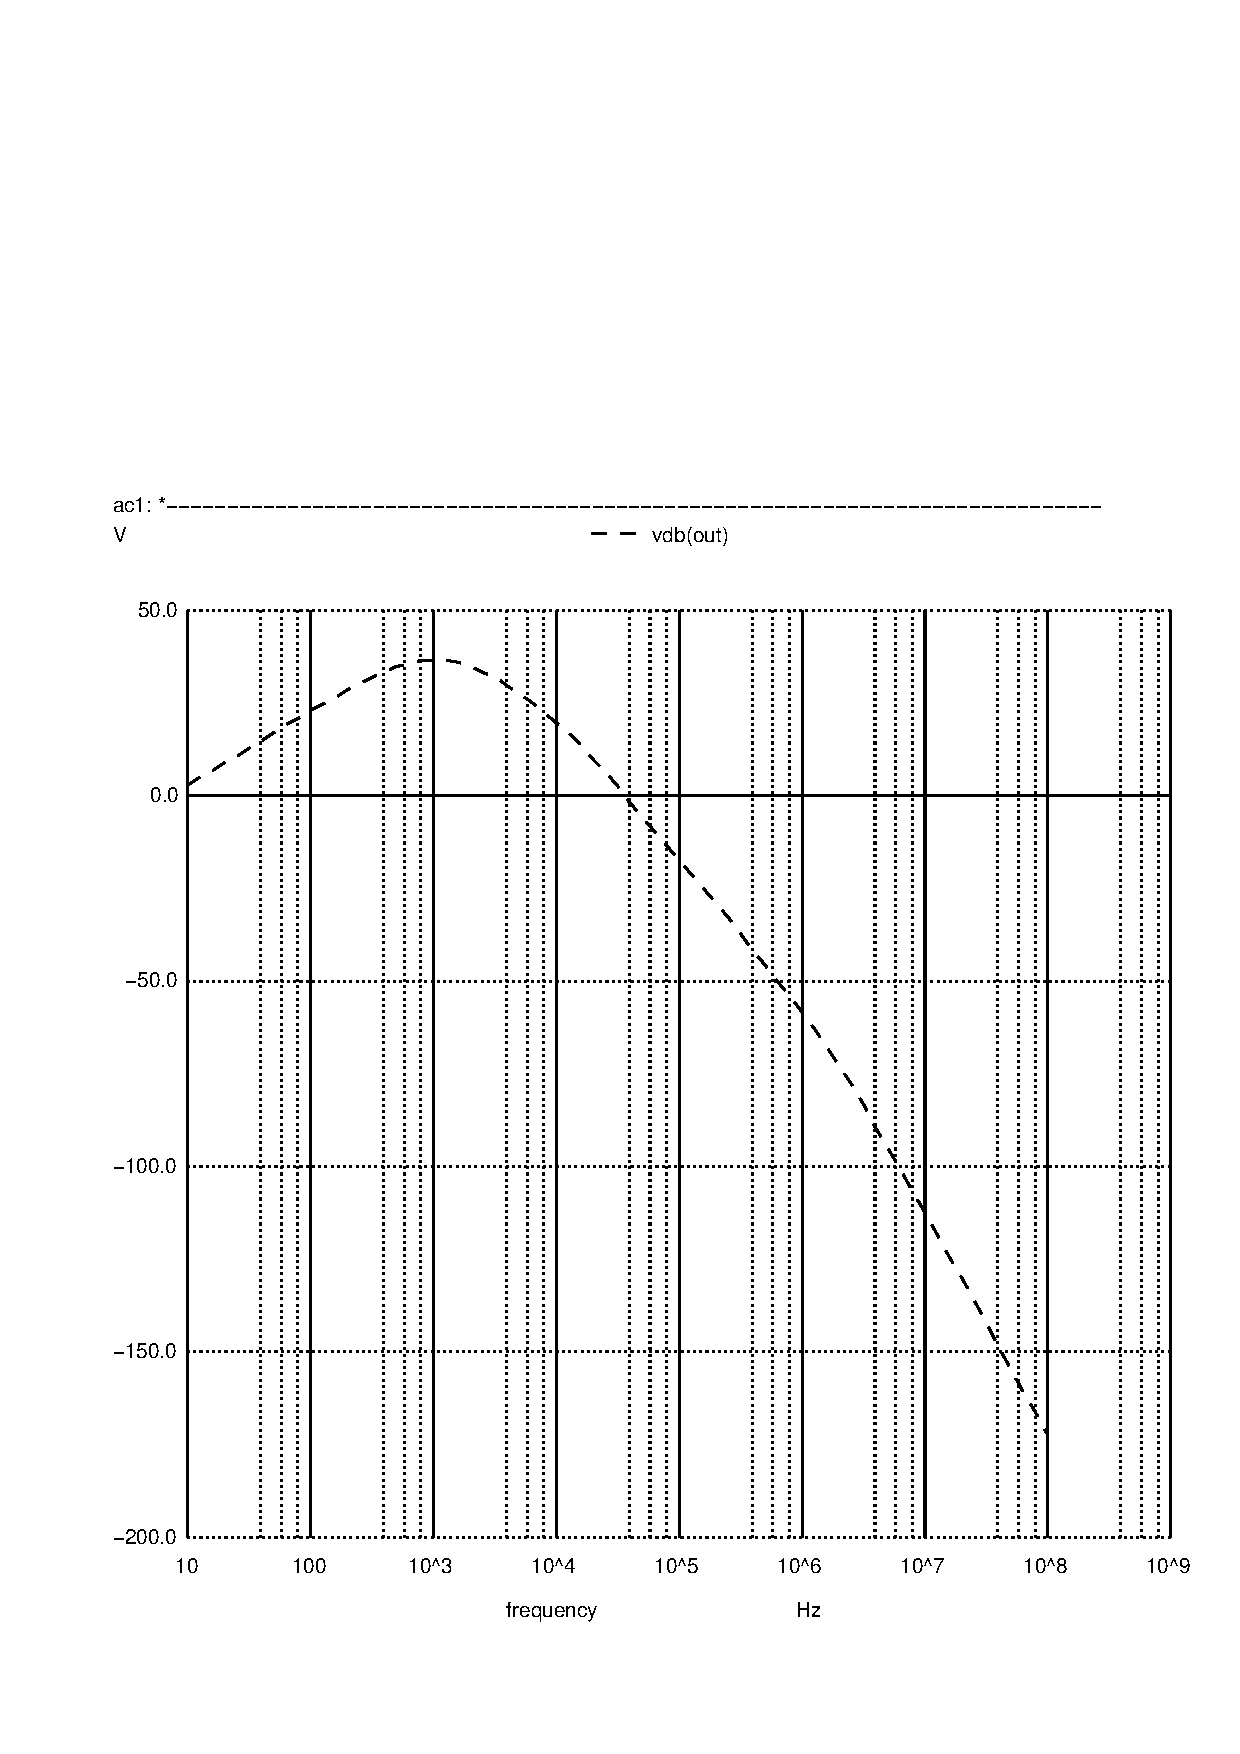
\includegraphics[width=\linewidth]{../sim/vo1f.pdf}
      \caption{Simulation Gain Frequency Response - $dB$}
    \endminipage\hfill
    \minipage{0.45\textwidth}
      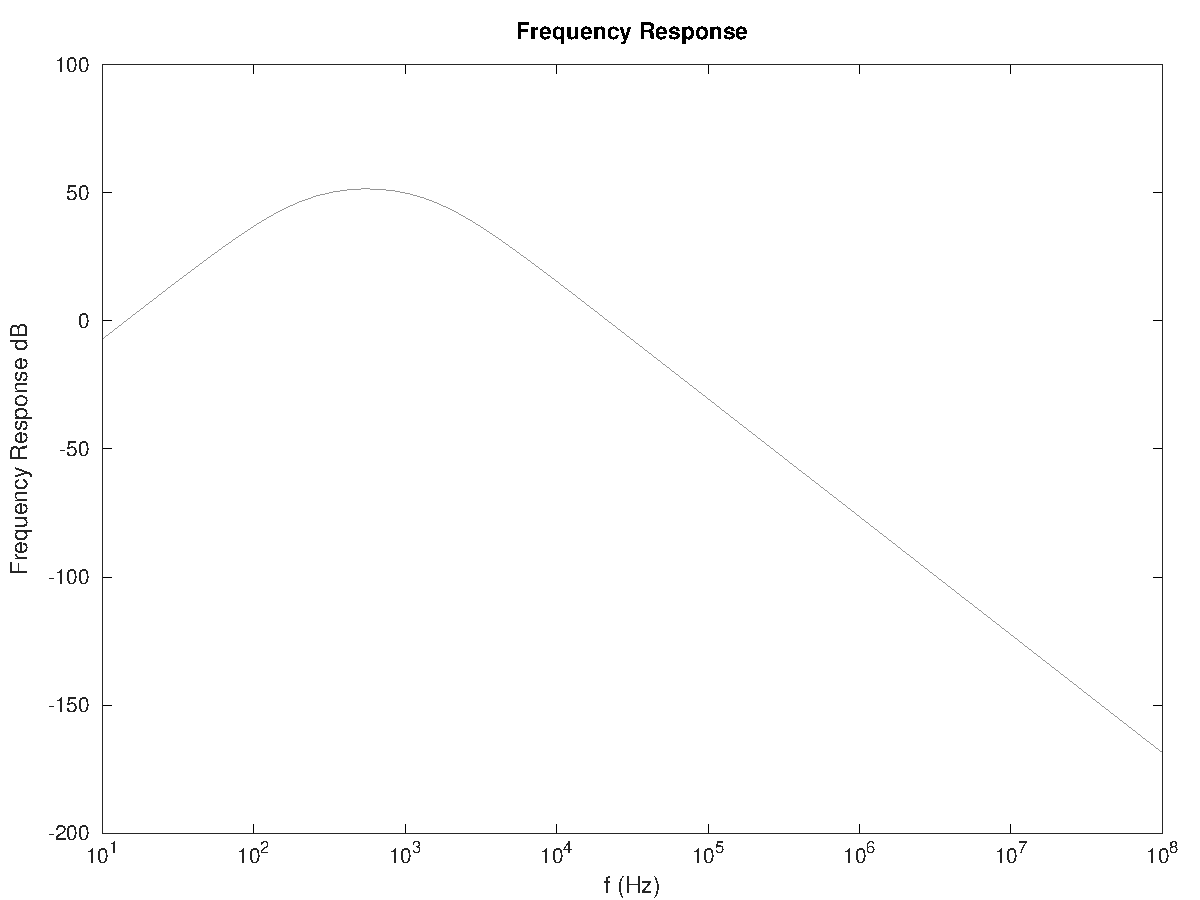
\includegraphics[width=\linewidth]{../mat/fresponse1.pdf}
      \caption{Theoretical Gain Frequency Response - $dB$}
    \endminipage\hfill
\end{figure}


\begin{figure}[H]
    \minipage{0.45\textwidth}
      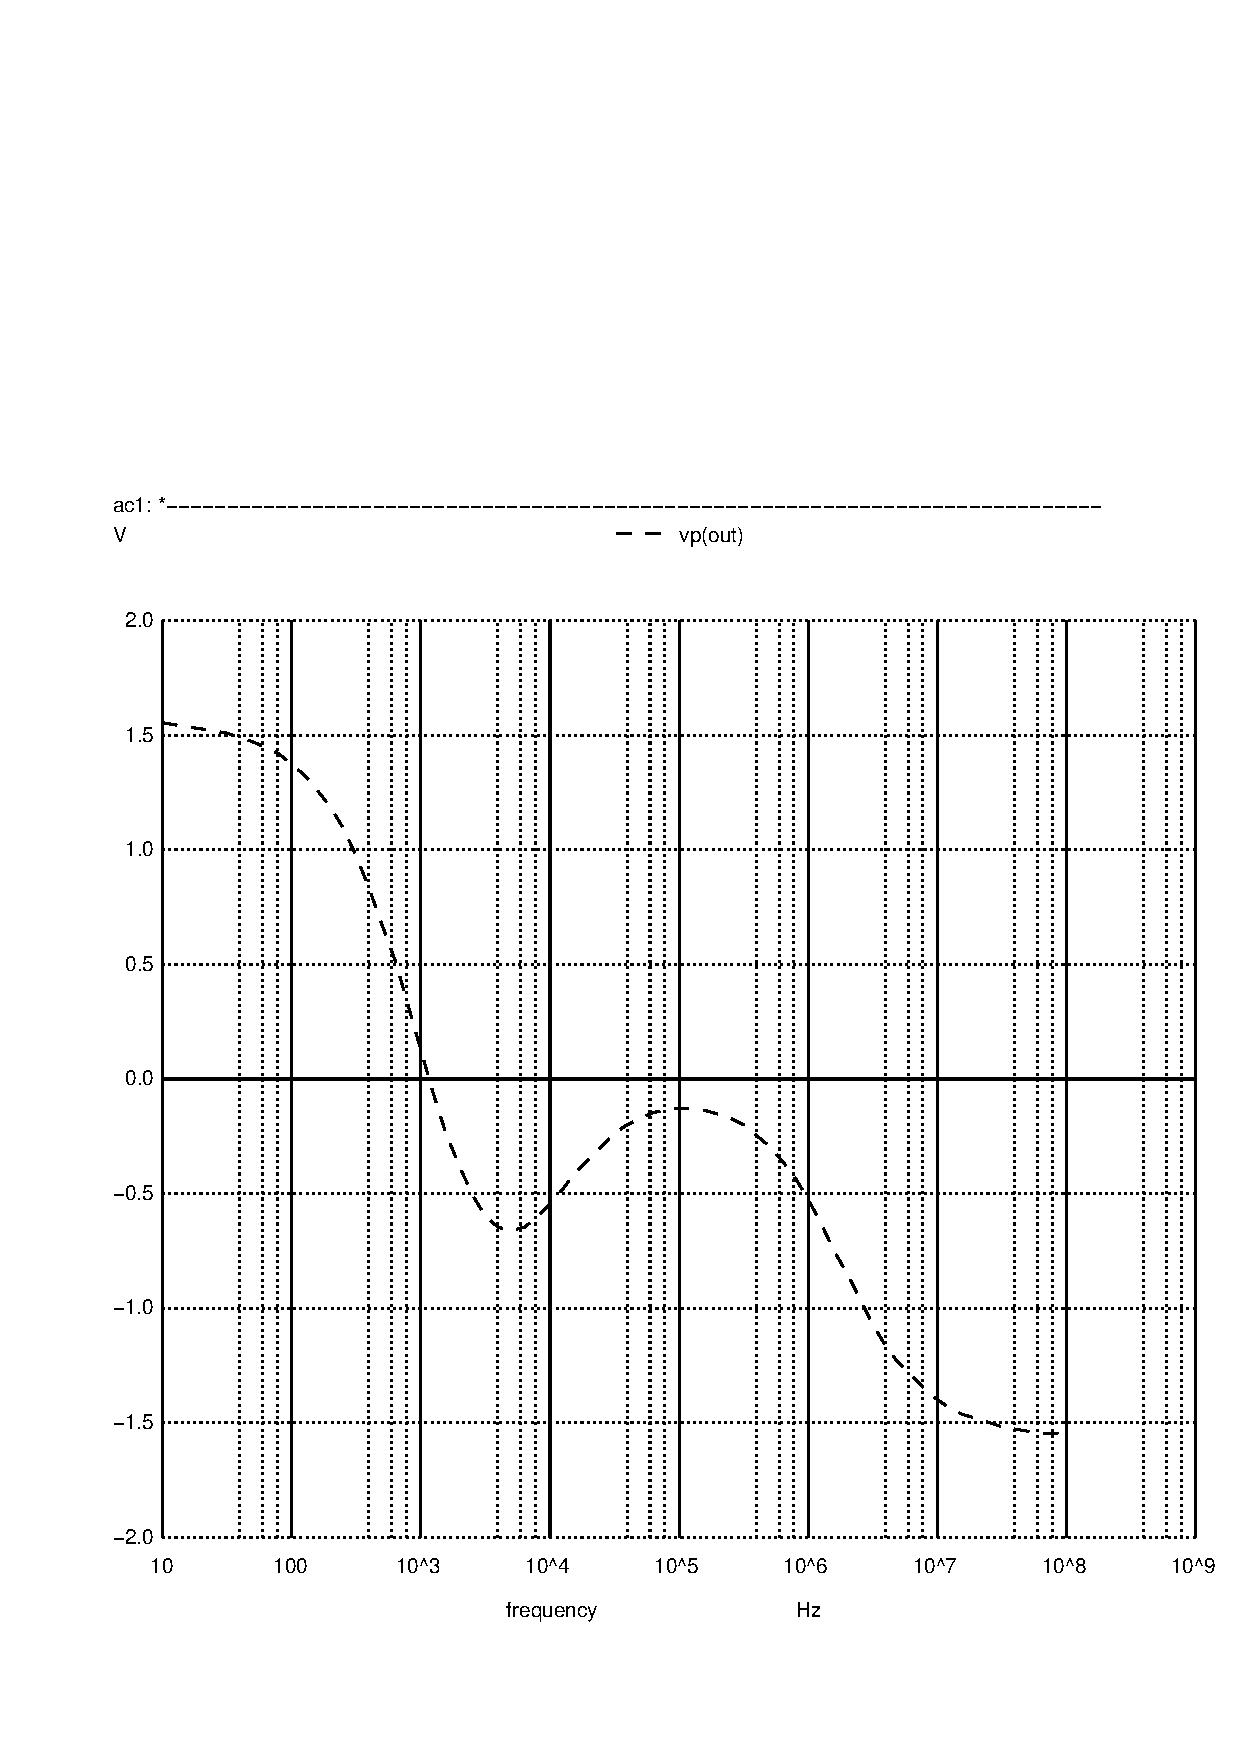
\includegraphics[width=\linewidth]{../sim/vo1p.pdf}
      \caption{Simulation Gain Frequency Response - Phase}
    \endminipage\hfill
    \minipage{0.45\textwidth}
      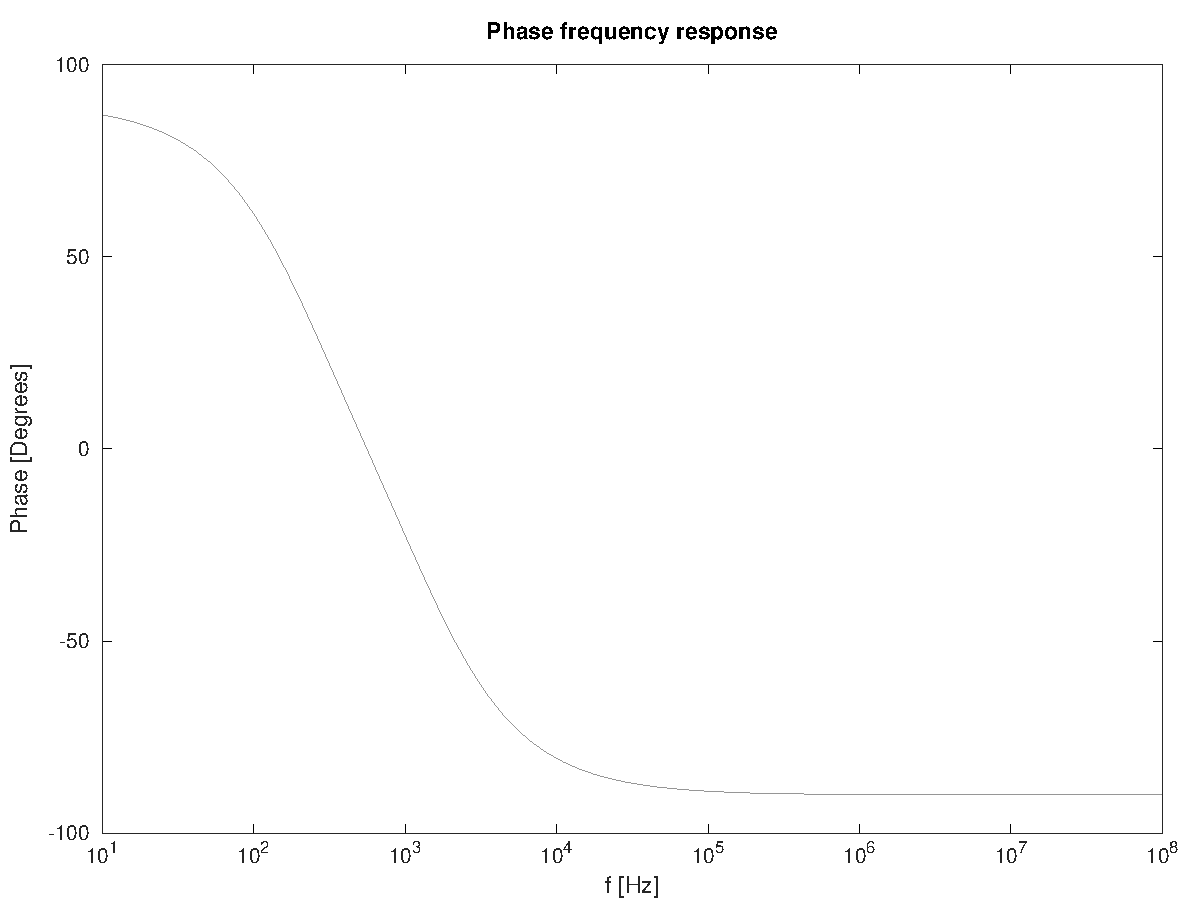
\includegraphics[width=\linewidth]{../mat/fresponse2.pdf}
      \caption{Theoretical Gain Frequency Response - Phase}
    \endminipage\hfill
\end{figure}


\begin{center}
  \begin{tabular}{ | c | c | }
    \hline    
    {\bf Name} & {\bf Value [$\Omega$]} \\ \hline
    inputimpedance & -9.99987e+02,7.233281e+02\\ \hline

  \end{tabular}
  \captionof{figure}{Simulation Input Impedance}
\end{center}

\begin{center}
  \begin{tabular}{ | c | c | }
    \hline    
    {\bf Name} & {\bf Value [$\Omega$]} \\ \hline
    Output Impedance & 345.125 + -475.63 j\\ \hline

  \end{tabular}
  \captionof{figure}{Simulation Output Impedance}
\end{center}

\begin{center}
  \begin{tabular}{ | c | c | }
    \hline    
    {\bf Name} & {\bf Value [$\Omega$]} \\ \hline
    Input Impedance & 5.000000e+02 \\ \hline 
Output Impedance & 2.396034e+02 \\ 

    \hline
  \end{tabular}
  \captionof{figure}{Theoretical Input and Output Impedances}
\end{center}
    \hline
  \end{tabular}
  \captionof{figure}{Merit Figure Table}
\end{center}

\begin{figure}[H]
    \minipage{0.45\textwidth}
      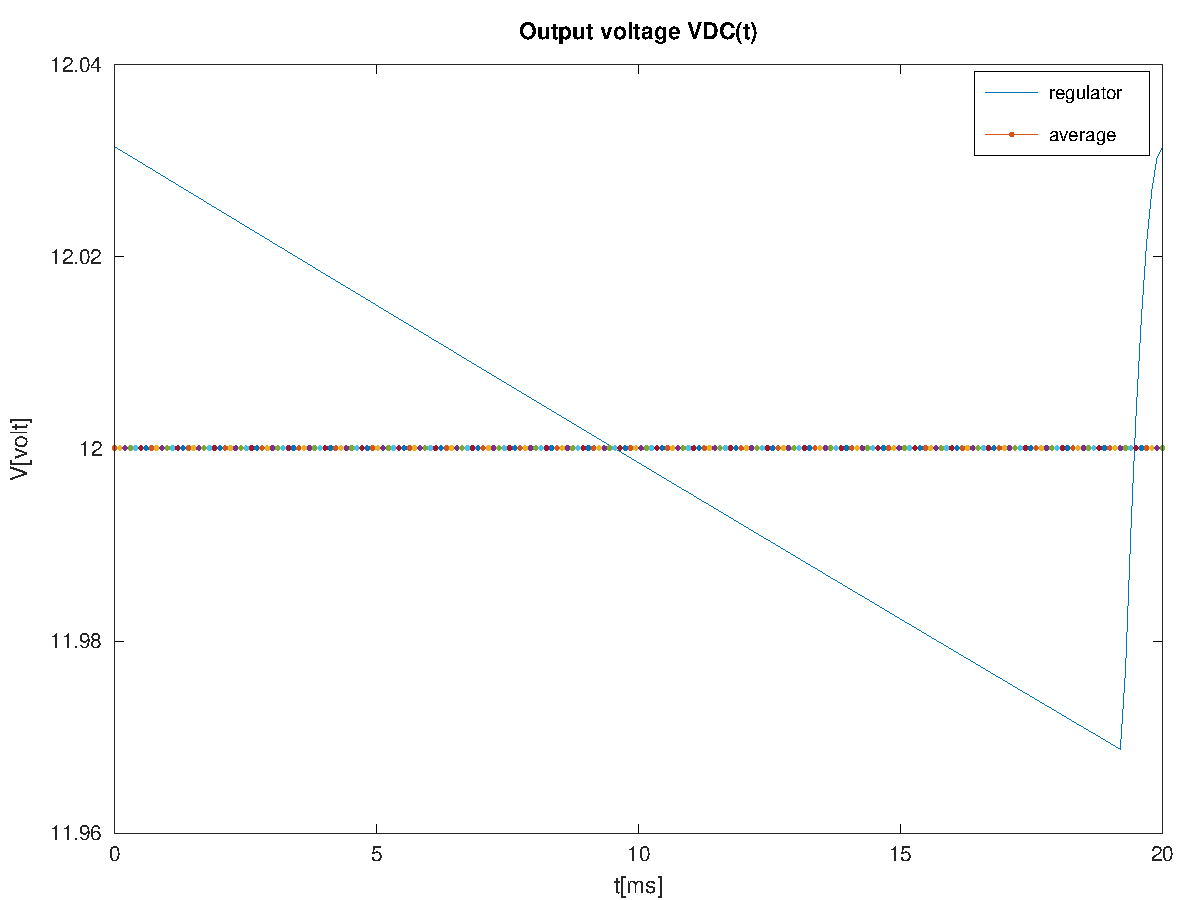
\includegraphics[width=\linewidth]{../mat/outputdc.pdf}
      \caption{Theoretical Output Voltage Level}
    \endminipage\hfill
    \minipage{0.45\textwidth}
      \includegraphics[width=\linewidth]{../sim/transient1.pdf}
      \caption{Simulation Output Voltage Level}
    \endminipage\hfill
\end{figure}

\begin{center}
  \begin{tabular}{ | c | c | }
    \hline    
    {\bf Name} & {\bf Value [V]} \\ \hline
    \input{../mat/ripple_octave}
    \hline
  \end{tabular}
  \captionof{figure}{Theoretical Ripple}
\end{center}

\begin{center}
  \begin{tabular}{ | c | c | }
    \hline    
    {\bf Name} & {\bf Value [V]} \\ \hline
    \input{ripple_tab}
  \end{tabular}
  \captionof{figure}{Simulation Ripple}
\end{center}

\begin{figure}[H]
    \minipage{0.45\textwidth}
      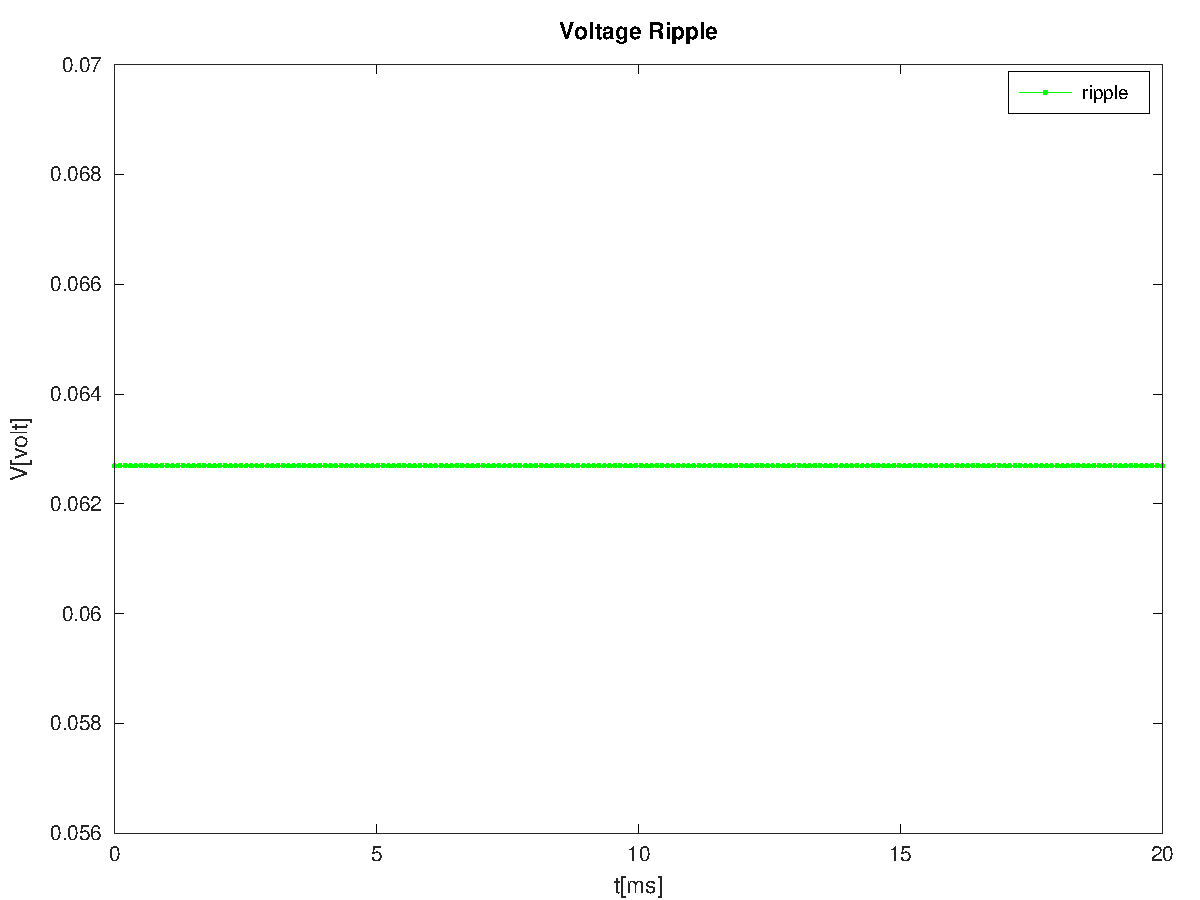
\includegraphics[width=\linewidth]{../mat/ripple.pdf}
      \caption{Theoretical Ripple}
    \endminipage\hfill
    \minipage{0.60\textwidth}
      \centering
      \begin{tabular}{ | c | c | }
      \hline    
      {\bf Ripple} & {\bf Value [V]} \\ \hline
      \input{ripple_tab}
      \end{tabular}
      \caption{Simulation Ripple}
    \endminipage\hfill
\end{figure}

\begin{figure}[H]
    \minipage{0.45\textwidth}
      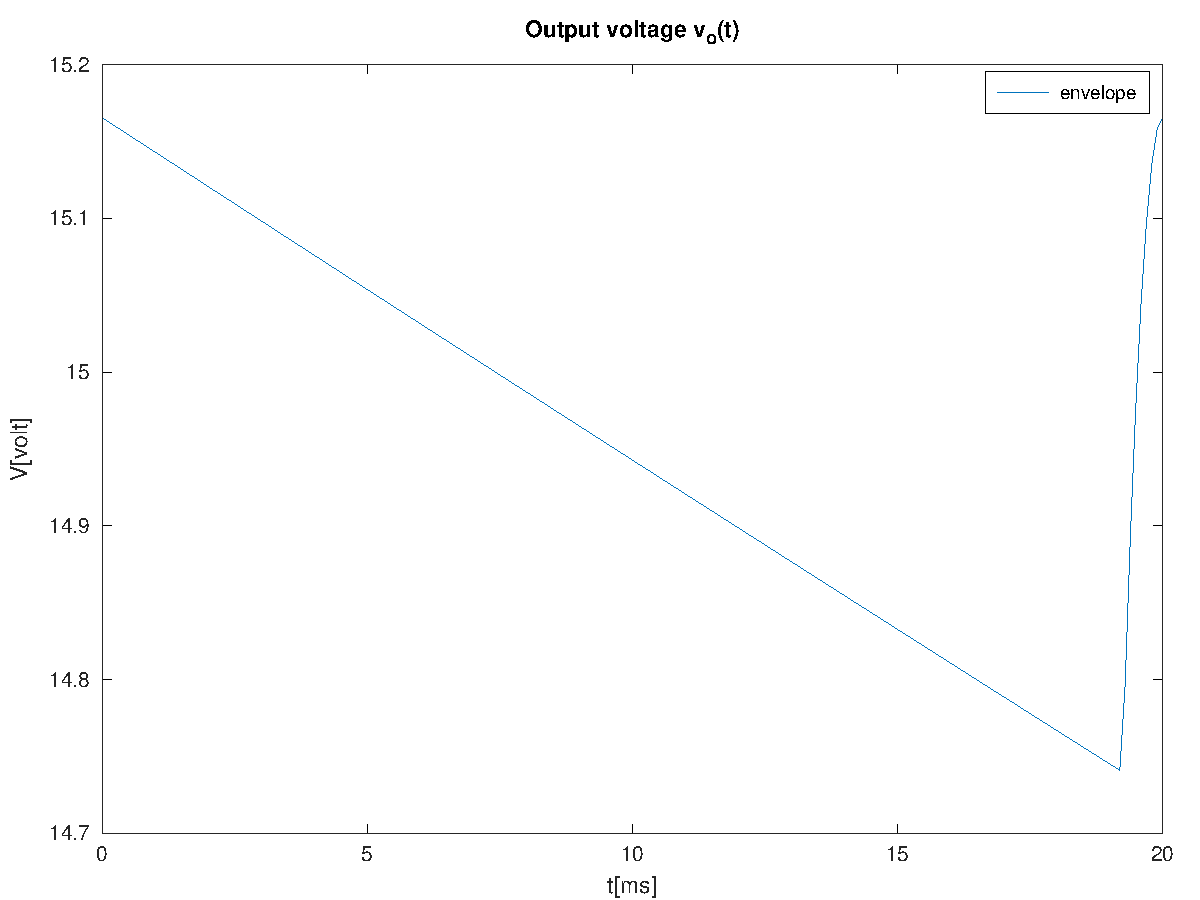
\includegraphics[width=\linewidth]{../mat/envelope.pdf}
      \caption{Theoretical Envelope Detector Voltage Level}
    \endminipage\hfill
    \minipage{0.45\textwidth}
      \includegraphics[width=\linewidth]{../sim/transient2.pdf}
      \caption{Simulation Envelope Detector Voltage Level}
    \endminipage\hfill
\end{figure}

\begin{figure}[H]
    \minipage{0.45\textwidth}
      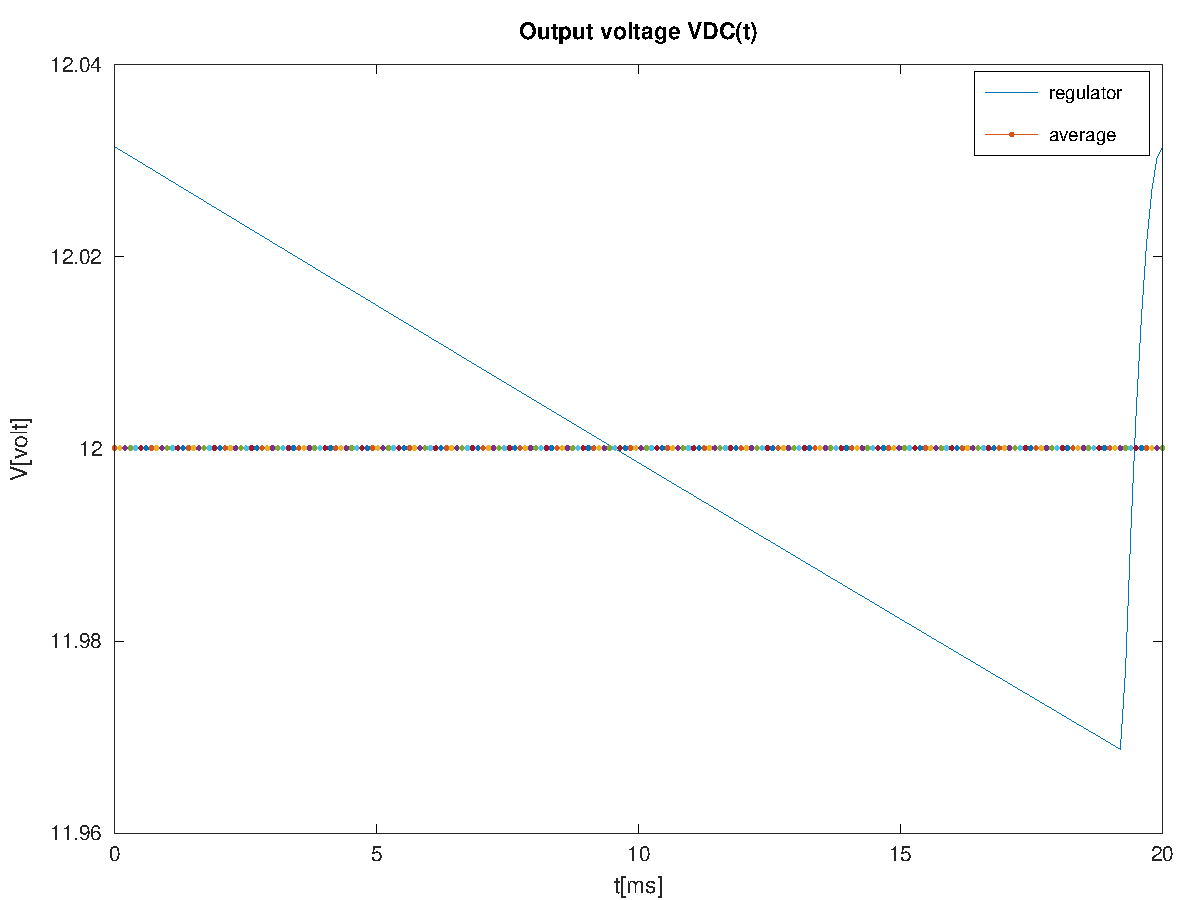
\includegraphics[width=\linewidth]{../mat/outputdc.pdf}
      \caption{Theoretical Voltage Regulator Voltage Level}
    \endminipage\hfill
    \minipage{0.45\textwidth}
      \includegraphics[width=\linewidth]{../sim/transient3.pdf}
      \caption{Simulation Voltage Regulator Voltage Level}
    \endminipage\hfill
\end{figure}

\begin{figure}[H]
    \minipage{0.45\textwidth}
      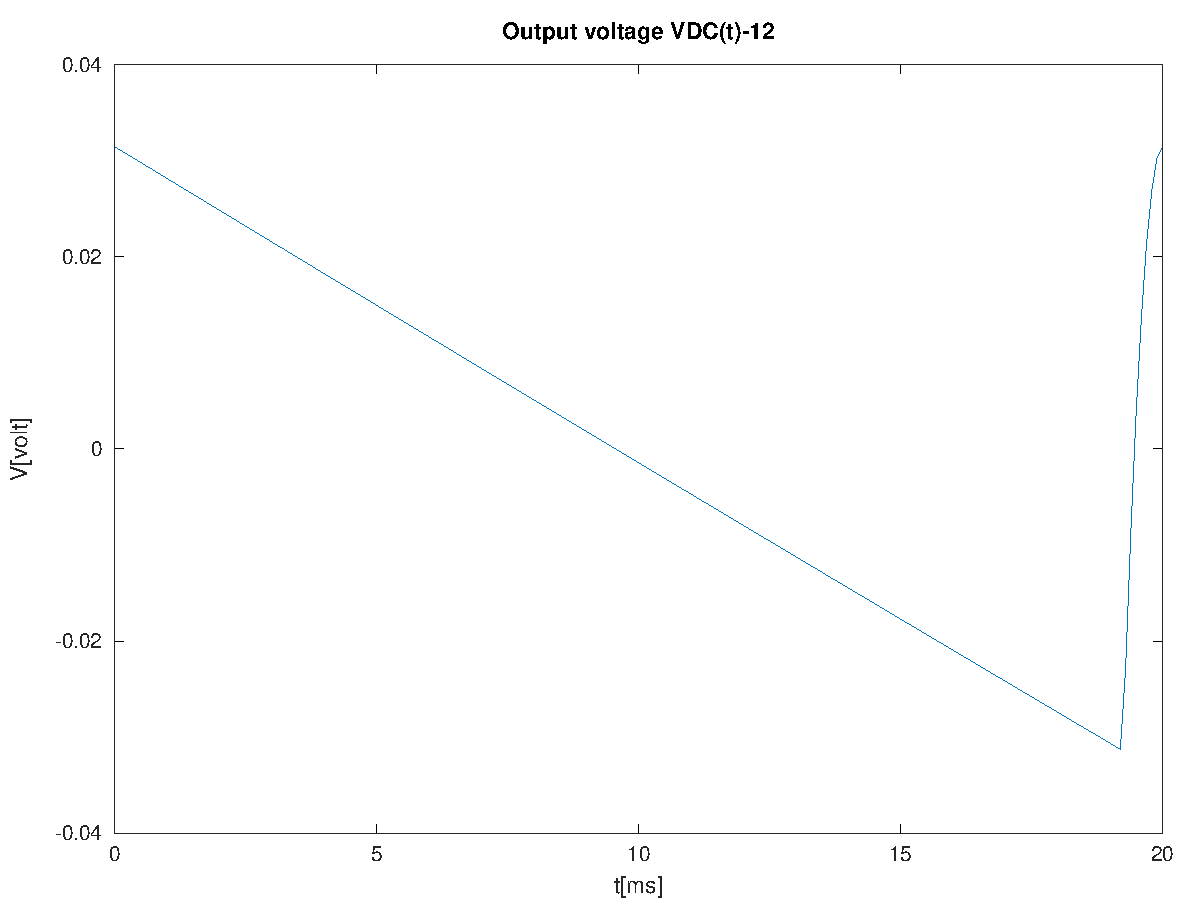
\includegraphics[width=\linewidth]{../mat/v012.pdf}
      \caption{Theoretical $v_0-12$ Voltage Level}
    \endminipage\hfill
    \minipage{0.45\textwidth}
      \includegraphics[width=\linewidth]{../sim/transient5.pdf}
      \caption{Simulation $v_0-12$ Voltage Level}
    \endminipage\hfill
\end{figure}